\newcommand{\econtexRoot}{.}

\documentclass[\econtexRoot/HAFiscal]{subfiles}
\onlyinsubfile{\externaldocument{\econtexRoot/HAFiscal}} % Get xrefs -- esp to apndx -- from main file; only works if main file has already been compiled

\begin{document}

\addcontentsline{toc}{section}{Appendices} % label the section "Appendices"

\hypertarget{Appendices}{} % Allows link to [url-of-paper]#Appendices
\ifthenelse{\boolean{Web}}{}{% Web version has no page headers
  \chead[Appendices]{Appendices}      % but PDF version does
  \appendixpage % Reset formatting for appendices
} 

%\hypertarget{Estimating-discount-factor-distributions-for-different-interest-rates}{}\par\section{Estimating discount factor distributions for different interest rates}
%\notinsubfile{\label{app:DF_R}}
%
%
%
%Figure~\ref{fig:LorenzPtsrobustnessR} shows the fit of the liquid wealth distribution for interest rates of $0.5$ percent and $1.5$ percent per quarter. In both cases, the estimation exactly matches the median liquid wealth to permanent income ratios for each education group listed in Panel~B of Table~\ref{tab:estimBetas}. 
%
% \begin{table}{th}
%   \begin{center}
%     \begin{tabular}{lccc}
%        %         \multicolumn{4}{l}{Panel (B) Estimation targets} \\ \midrule
%        %         & Dropout & Highschool & College \\ \midrule
%        %         Median LW/PI (data) & 4.64 & 30.2 & 112.8 \\ 
%        %         Median LW/PI (model, $R = 1.005$) & 4.64 & 30.2 & 112.8 \\	
%        %         Median LW/PI (model, $R = 1.01$) & 4.64 & 30.2 & 112.8 \\
%        %         Median LW/PI (model, $R = 1.015$) & 4.64 & 30.2 & 112.8 \\ \bottomrule
%        %       \end{tabular} \\ \\ 
%        %         \end{center}	
%        %         \end{table}
%
%\begin{figure}[th]
%  \begin{center}
%    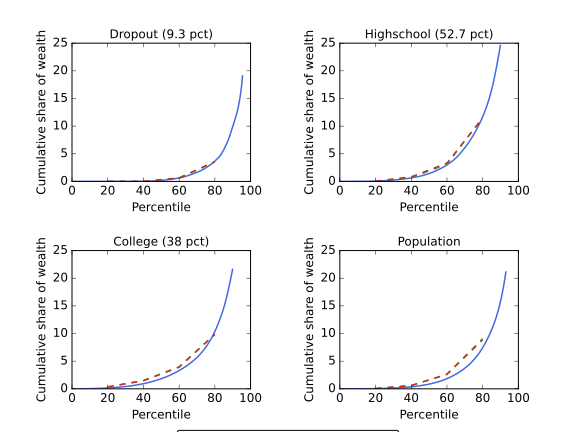
\includegraphics[width=.9\textwidth]{\econtexRoot/Figures/LorenzPoints_robustness_R}
%    \caption{Distributions of liquid wealth within each educational group and for the whole population from the 2004 Survey of Consumer Finance and from the estimated model for different values of the interest rate, $R$.}
%    \notinsubfile{\label{fig:LorenzPtsrobustnessR}}
%  \end{center}
%\end{figure}
%
%
%
%\FloatBarrier


%\subfile{Robustness}
\newcommand{\econtexRoot}{.}

\documentclass[\econtexRoot/HAFiscal]{subfiles}
\onlyinsubfile{\externaldocument{\econtexRoot/HAFiscal}} % Get xrefs -- esp to apndx -- from main file; only works if main file has already been compiled

\begin{document}
	
\FloatBarrier
\hypertarget{hank_appendix}{}\par\section{Details of the HANK and SAM Model}
\notinsubfile{\label{sec:hank_appendix}}


\subsection{Households}

The household block follows closely to the main text with a few exceptions. First, the splurge only occurs out of equilibrium---that is, the steady state of the model is calculated without the splurge behavior. Second, the level of permanent income of all newborns is equal to one. Furthermore, all households face the same employment to unemployment and unemployment to employment probabilities. The probabilities are calibrated to the transition probabilities of high school graduates from the main text. Lastly, following the notation of \cite{Auclert2020}, $r^{a}_{t}$ will denote the economy wide ex-ante real interest rate.


\subsection{Goods Market}

There is a continuum of  monopolistically competitive intermediate goods producers indexed by $j \in [0,1]$ who produce intermediate goods $Y_{jt}$ to be sold to a final goods producer at price $P_{jt}$. We assume intermediate goods producers consume all profits each period.  

\subsubsection{Final Goods Producer}

A perfectly competitive final goods producer purchases intermediate goods $Y_{jt}$ for $j \in [0,1]$, from intermediate goods producers at price $P_{jt}$ and produces a final good $Y_{t}$ according to a CES production function given by 
$$ Y_{t} = \left(\int_{0}^{1} Y_{jt}^{\frac{\epsilon_{p}-1}{\epsilon_{p}}}\, dj\right)^{\frac{\epsilon_{p}}{\epsilon_{p}-1}},$$ 
where $\epsilon_{p}$ is the elasticity of substitution.

Given $P_{jt}$, the price of intermediate good $j$, the final goods producer maximizes profits by solving:
$$ \max_{Y_{jt}} P_{t} \left(\int_{0}^{1} Y_{jt}^{\frac{\epsilon_{p}-1}{\epsilon_{p}}}\, dj\right)^{\frac{\epsilon_{p}}{\epsilon_{p}-1}} - \int_{0}^{1} P_{jt} Y_{jt} ,\ dj.$$ 
%\vspace{.2cm}

The first order condition leads to demand for good $j$ given by
$$Y_{jt} = \left(\frac {P_{jt}}{P_{t}}\right)^{- \epsilon_{p}} Y_{t},$$
and the price index
$$P_{t} = \left(\int_{0}^{1} P_{jt}^{1-\epsilon_{p}}\,dj \right )^{\frac{1}{1-\epsilon_{p}}}.$$


\subsubsection{Intermediate Goods Producers}

Intermediate goods producers produce according to a production function linear in labor~$L_{t}$: 
$$Y_{jt} =  Z L_{jt},$$ 
where $Z$ is total factor productivity.
%\vspace{.3cm}
  
Each intermediate goods producer hires labor~$L_{t}$ from a labor agency at cost~$h_{t}$. Given the cost of labor, each intermediate goods producer chooses~$P_{jt}$ to maximize its profits facing price stickiness a la \cite{Rotemberg1982}. HANK models with sticky prices produce countercyclical profits which combined with households with high MPCs can lead to countercyclical consumption responses out of dividends. Therefore, we simply assume that intermediate goods producers consume all profits rather than distributing them to households. We therefore abstract from consumption behavior in response to firm profits. Intermediate goods producers maximize profits by solving:
$$J_{t}\left(P_{jt}\right) = \max_{\{P_{jt}\}} \left\{\frac{P_{jt}Y_{jt}}{P_{t}} - h_{t} L_{jt} -  \frac{\varphi}{2}\left( \frac{P_{jt} - P_{jt-1}}{P_{jt-1}} \right)^{2} Y_{t}  + J_{t+1}\left(P_{jt+1}\right) \right\},$$ 

where $\varphi$ determines the cost of adjusting the price and, hence, the degree of price stickiness. 

The problem can be rewritten as the standard New Keynesian maximization problem:
$$\max_{\{P_{jt}\}} \mathrm{E}_{t}\left[\sum_{s=0}^{\infty}  M_{t,t+s} \left( \left( \frac{P_{jt+s}}{P_{t+s}} - MC_{t+s}\right)Y_{jt+s} -  \frac{\varphi}{2}\left( \frac{P_{jt+s}}{P_{jt+s-1}} - 1\right)^{2} Y_{t+s} \right)\right],$$ 
where $MC_{t} = \frac{h_{t}}{Z}$.

Given that all firms face the same adjustment costs, there exists a symmetric equilibrium where all firms choose the same price with $P_{jt}=P_{t}$ and $Y_{jt}=Y_{t}$.

The resulting Phillips Curve is
$$ \epsilon_{p} MC_{t} = \epsilon_{p} - 1 + \varphi ( \Pi_{t} -1) \Pi_{t} - M_{t,t+1} \varphi (\Pi_{t+1} -1 ) \Pi_{t+1} \frac{Y_{t+1}}{Y_{t}}$$
where $\Pi_{t} = \frac{P_{t}}{P_{t+1}}$. 

\subsection{Labor market}

A risk neutral labor agency sells labor $N_{t}$ to intermediate goods producers at cost~$h_{t}$ by hiring households at the wage~$w_t$. To hire households, the labor agency posts vacancies~$v_{t}$ that are filled with probability~$\phi_{t}$. Household's search is random. Following~\cite{Bardoczy2022}, we assume the labor agency cannot observe the labor productivity of individual households. Instead, the agency can only observe the average productivity of all employed workers which is always equal to one. 

\textbf{Labor agency.} The labor agency determines how many vacancies to post and how much labor to sell by solving the following problem: 
$$J_{t}(N_{t-1})  = \max_{N_{t},v_{t}} \left\{( h_{t} - w_{t}) N_{t}- \kappa v_{t} + \mathrm{E_{t}}\left[ \frac{J_{t+1}(N_{t})}{1 + r^{a}_{t}}\right]\right\},$$
subject to
$$ N_{t} = (1-\omega)N_{t-1} + \phi_{t} v_{t}.$$ 

The parameters $\kappa$ and $\omega$ are, respectively, the cost of posting a vacancy, and the job separation rate. 

The resulting job creation curve is:
$$ \frac{\kappa}{\phi_{t}}  = (h_{t} - w_{t})+  (1-\omega)\mathrm{E_{t}}\left[   \frac{\kappa}{(1+r^{a}_{t}) \phi_{t+1}} \right].$$

\textbf{Matching.} Matching between households and the labor agency follows a Cobb-Douglas matching function:
$$m_{t} = \chi e_{t}^{\alpha} v_{t}^{1-\alpha},$$ 
where $m_{t}$ is the mass of matches, $e_{t}$ is the mass of job searchers, $\alpha$ is the matching function elasticity, and $\chi$ is a matching efficiency parameter.

The vacancy filling probability $\phi_{t}$ and the job finding probabilities $\eta_{t}$ evolve according to:
$$\eta_{t} = \chi \Theta_{it}^{1-\alpha} $$
%$$\eta_{t}(X) = \chi q(X) \Theta_{it}^{1-\alpha} $$
$$ \phi_{t} = \chi \Theta_{t}^{-\alpha} $$ 
where $\Theta_{t} = \frac{v_{t}}{e_{t}}$ is labor market tightness.

\textbf{Wage Determination.} Similar to \cite{Gornemann2021} and \cite{Blanchard2010}, we assume the real wage follows the rule:
$$log\left(\frac{w_{t}}{w_{ss}}\right)  = \phi_w log\left( \frac{ w_{t-1}}{ w_{ss}} \right) +   (1 - \phi_w) log\left( \frac{N_{t}}{N_{ss}}\right),$$
where $\phi_w$ dictates the extent of real wage rigidity. 

\subsection{Fiscal Policy}

The government issues long term bonds $B_{t}$ at price $q^{b}_{t}$ in period $t$ that pays $\delta^{s}$ in period $t+s+1$ for $s \in \{0,1,2,\ldots\}$.

The bond price satisfies the no arbitrage condition:
$$q^{b}_{t} = \frac{ 1  + \delta \mathrm{E}_{t}[q^{b}_{t+1}]}{1+r^{a}_{t}}.$$ 

The government finances its expenditures with debt and taxes and faces a budget constraint given by: 
$$ (1 + \delta q^{b}_{t})B_{t-1} + G_{t}  + S_{t} = \tau_{t} w_{t} N_{t}+ q^{b}_{t}B_{t},$$
where $S_{t}$ are payments for unemployment insurance and other transfers.

For all stimulus policies excluding the tax cuts, we follow \cite{Auclert2020} and let the tax rate adjusts to stabilize the debt to GDP ratio:
$$\tau_{t} - \tau_{ss} = \phi_{B} q^{b}_{ss} \frac{B_{t-1} - B_{ss} }{Y_{ss}}$$
where $\phi_{B}$ governs the speed of adjustment. 

For the tax cuts, we assume:
$$G_{t} - G_{ss} = \phi_{G} q^{b}_{ss} \frac{B_{t-1} - B_{ss} }{Y_{ss}}$$
where $\phi_{G}$ governs the speed of adjustment of government spending in response to debt. 

\subsection{Monetary Policy}

The central bank follows a simple Taylor rule where it only responds to inflation: 
$$i_{t} = r^{*} +\phi_{\pi} \pi_{t},$$ 
where $\phi_{\pi}$ is the coefficient on inflation. Inflation is given by $\pi_t = P_t/P_{t-1}-1$, and~$r^{*}$ is the steady state interest rate. 

\subsection{Equilibrium}

An equilibrium in this economy is a sequence of: 
\begin{itemize}[label=--]
	\item Policy Functions $\left( c_{it}(m) \right )_{t=0}^{\infty}$ normalized by permanent income.
	\item Prices $ \left( r^{a}_{t+1}, i_{t}, q^{b}_{t},  w_{t}, h_{t} , \pi_{t} , \tau_{t} \right) _{t=0}^{\infty}$.
	\item Aggregates $ \left(C_{t}, Y_{t} , N_{t},   \Theta_{t},  B_{t} , A_{t}  \right)_{t=0}^{\infty}$.
\end{itemize}

Such that: 
\begin{itemize}[label=--]
\item $\left(c_{it}(m)\right)_{t=0}^{\infty}$  solves the household's maximization problem given $\left( w_{t}, \eta_{t},  r^{a}_{t} , \tau_{t} \right)_{t=0}^{\infty}$.
\item The final goods producer and intermediate goods producers maximize their objective functions.
\item The nominal interest rate is set according to the central bank's Taylor rule.
\item The tax rate is determined by the fiscal rule and the government budget constraint holds.
\item The value of assets is equal to the value of government bonds:
 $$A_t =  q^{b}_{t}B_{t}.$$
\item The goods market clears\footnote{Note if profits were not held by firms then the goods market condition would be $ C_{t}  + G_{t}  = Y_{t} -  \kappa v_{t} - \frac{\varphi}{2}\left( \frac{P_{t}}{P_{t-1}} - 1\right)^{2} Y_{t}  $.  In particular, since firm profits are $D_{t} = Y_{t} -  w_{t} N_{t}  - \kappa v_{t} - \frac{\varphi}{2}\left( \frac{P_{t}}{P_{t-1}} - 1\right)^{2} Y_{t} $, then the goods market condition would become $ C_{t}  + G_{t}  =w_{t} N_{t}  + D_{t} = Y_{t} -  \kappa v_{t} - \frac{\varphi}{2}\left( \frac{P_{t}}{P_{t-1}} - 1\right)^{2} Y_{t}  $. }: 
$$ C_{t}  = w_{t} N_{t}  + G_{t},$$
where $C_{t} \equiv  \int_{0}^{1} \textbf{c}_{it} \, di$. 
\item The labor demand of intermediate goods producers equals labor supply of labor agency:
$$ L_{t} =  N_{t}.$$ 
\end{itemize}

%\input{\TableDir/Calibration.tex}


\begin{table}
\begin{center}
\renewcommand{\arraystretch}{1.6}
\caption{Calibration}\label{table:Calibration}
\makebox[\textwidth]{\begin{tabular}{l c c l}
Description & Parameter & Value & Source/Target \\ \hline
Elasticity of Substitution & $\epsilon_{p}$ & 6 & Standard \\
Price Adjustment Costs & $\varphi$ & 96.9 & \cite{Ravn2017} \\
Vacancy Cost & $\kappa$ & 0.056 & $\frac{\kappa}{w\phi} = 0.071$ \\
Job Separation Rate & $\omega$ & 0.092 & Match $\pi(eu)$ for Highschool group \\
Matching Elasticity & $\alpha$ & 0.65 & \cite{Ravn2017} \\
Job Finding Probability & $\eta_{ss}$ & 0.67 & $\pi(ue)$ in section~\ref{sec:calib} \\
Vacancy Filling Rate & $\phi_{ss}$ & 0.71 & den Haan et al. (\citeyear{DenHaan2000}) \\
Real Wage Rigidity parameter & $\phi_{w}$ & 0.837 & Gornemann et al. (\citeyear{Gornemann2021}) \\
Government Spending & $G$ & 0.38 & Gov. budget constraint \\
Decay rate of Gov. Coupons & $\delta$ & 0.95 & 5 Year Maturity of Debt \\
Response of Tax Rate to Debt & $\phi_{B}$ & 0.015 & Auclert et al. (\citeyear{Auclert2020}) \\
Taylor Rule Inflation Coefficient & $\phi_{\pi}$ & 1.5 & Standard \\ \hline
\end{tabular}}
\end{center}
\end{table}

\section{Calibration of Non-Household Blocks }

The elasticity of substitution is set to 6, and the price adjustment cost parameter is set to 96.9 as in \cite{Ravn2017}.
The vacancy cost is set to 7\% of the real wage as in \cite{Christiano2016}.\footnote{The range of plausible values lie between $4\%$ and $14\%$ \cite{Silva2009}} The matching elasticity is 0.65 following \cite{Ravn2017}. The job separation rate is set to 0.092. As in section~\ref{sec:calib}, we set the job finding probability in the steady state for the unemployed $\eta_{ss}$ to 0.67. Along with the job separation rate, this gives a probability of transitioning from employment to unemployment within a quarter of $3.1$ percent which is the value we use for the Highschool group in section~\ref{sec:calib}. The quarterly vacancy filling rate is 0.71 as in \cite{DenHaan2000} (and together with our other choices, this pins down the matching efficiency $\chi$). The degree of wage rigidity $\phi_w$ is set to 0.837 following \cite{Gornemann2021}. The tax rate is set to 0.3 and government spending is set to clear the government budget constraint. The parameters that dictate the speed of fiscal adjustment, $\phi_{B}$ and $\phi_{G}$, are set to 0.015, the lower bound of the estimates in \cite{Auclert2020}.\footnote{The speed of adjustment parameter is set to the lower bound to ensure that the policies evaluated in the HANK and SAM model are almost entirely deficit financed.} Furthermore, the decay rate of government coupons is set to $\delta = 0.95$ to match a maturity of 5 years.\footnote{The duration of bonds in the model is $\frac{(1+r)^4}{(1+r)^4 - \delta}$} Finally, the Taylor rule coefficient on inflation is set to the standard value of $\phi_{\pi}=1.5$. 


\ifthenelse{\boolean{Web}}{}{
\end{document} \endinput
}



\ifthenelse{\boolean{Web}}{}{
\end{document} \endinput
}

